\begin{figure}[H]
    \centering
    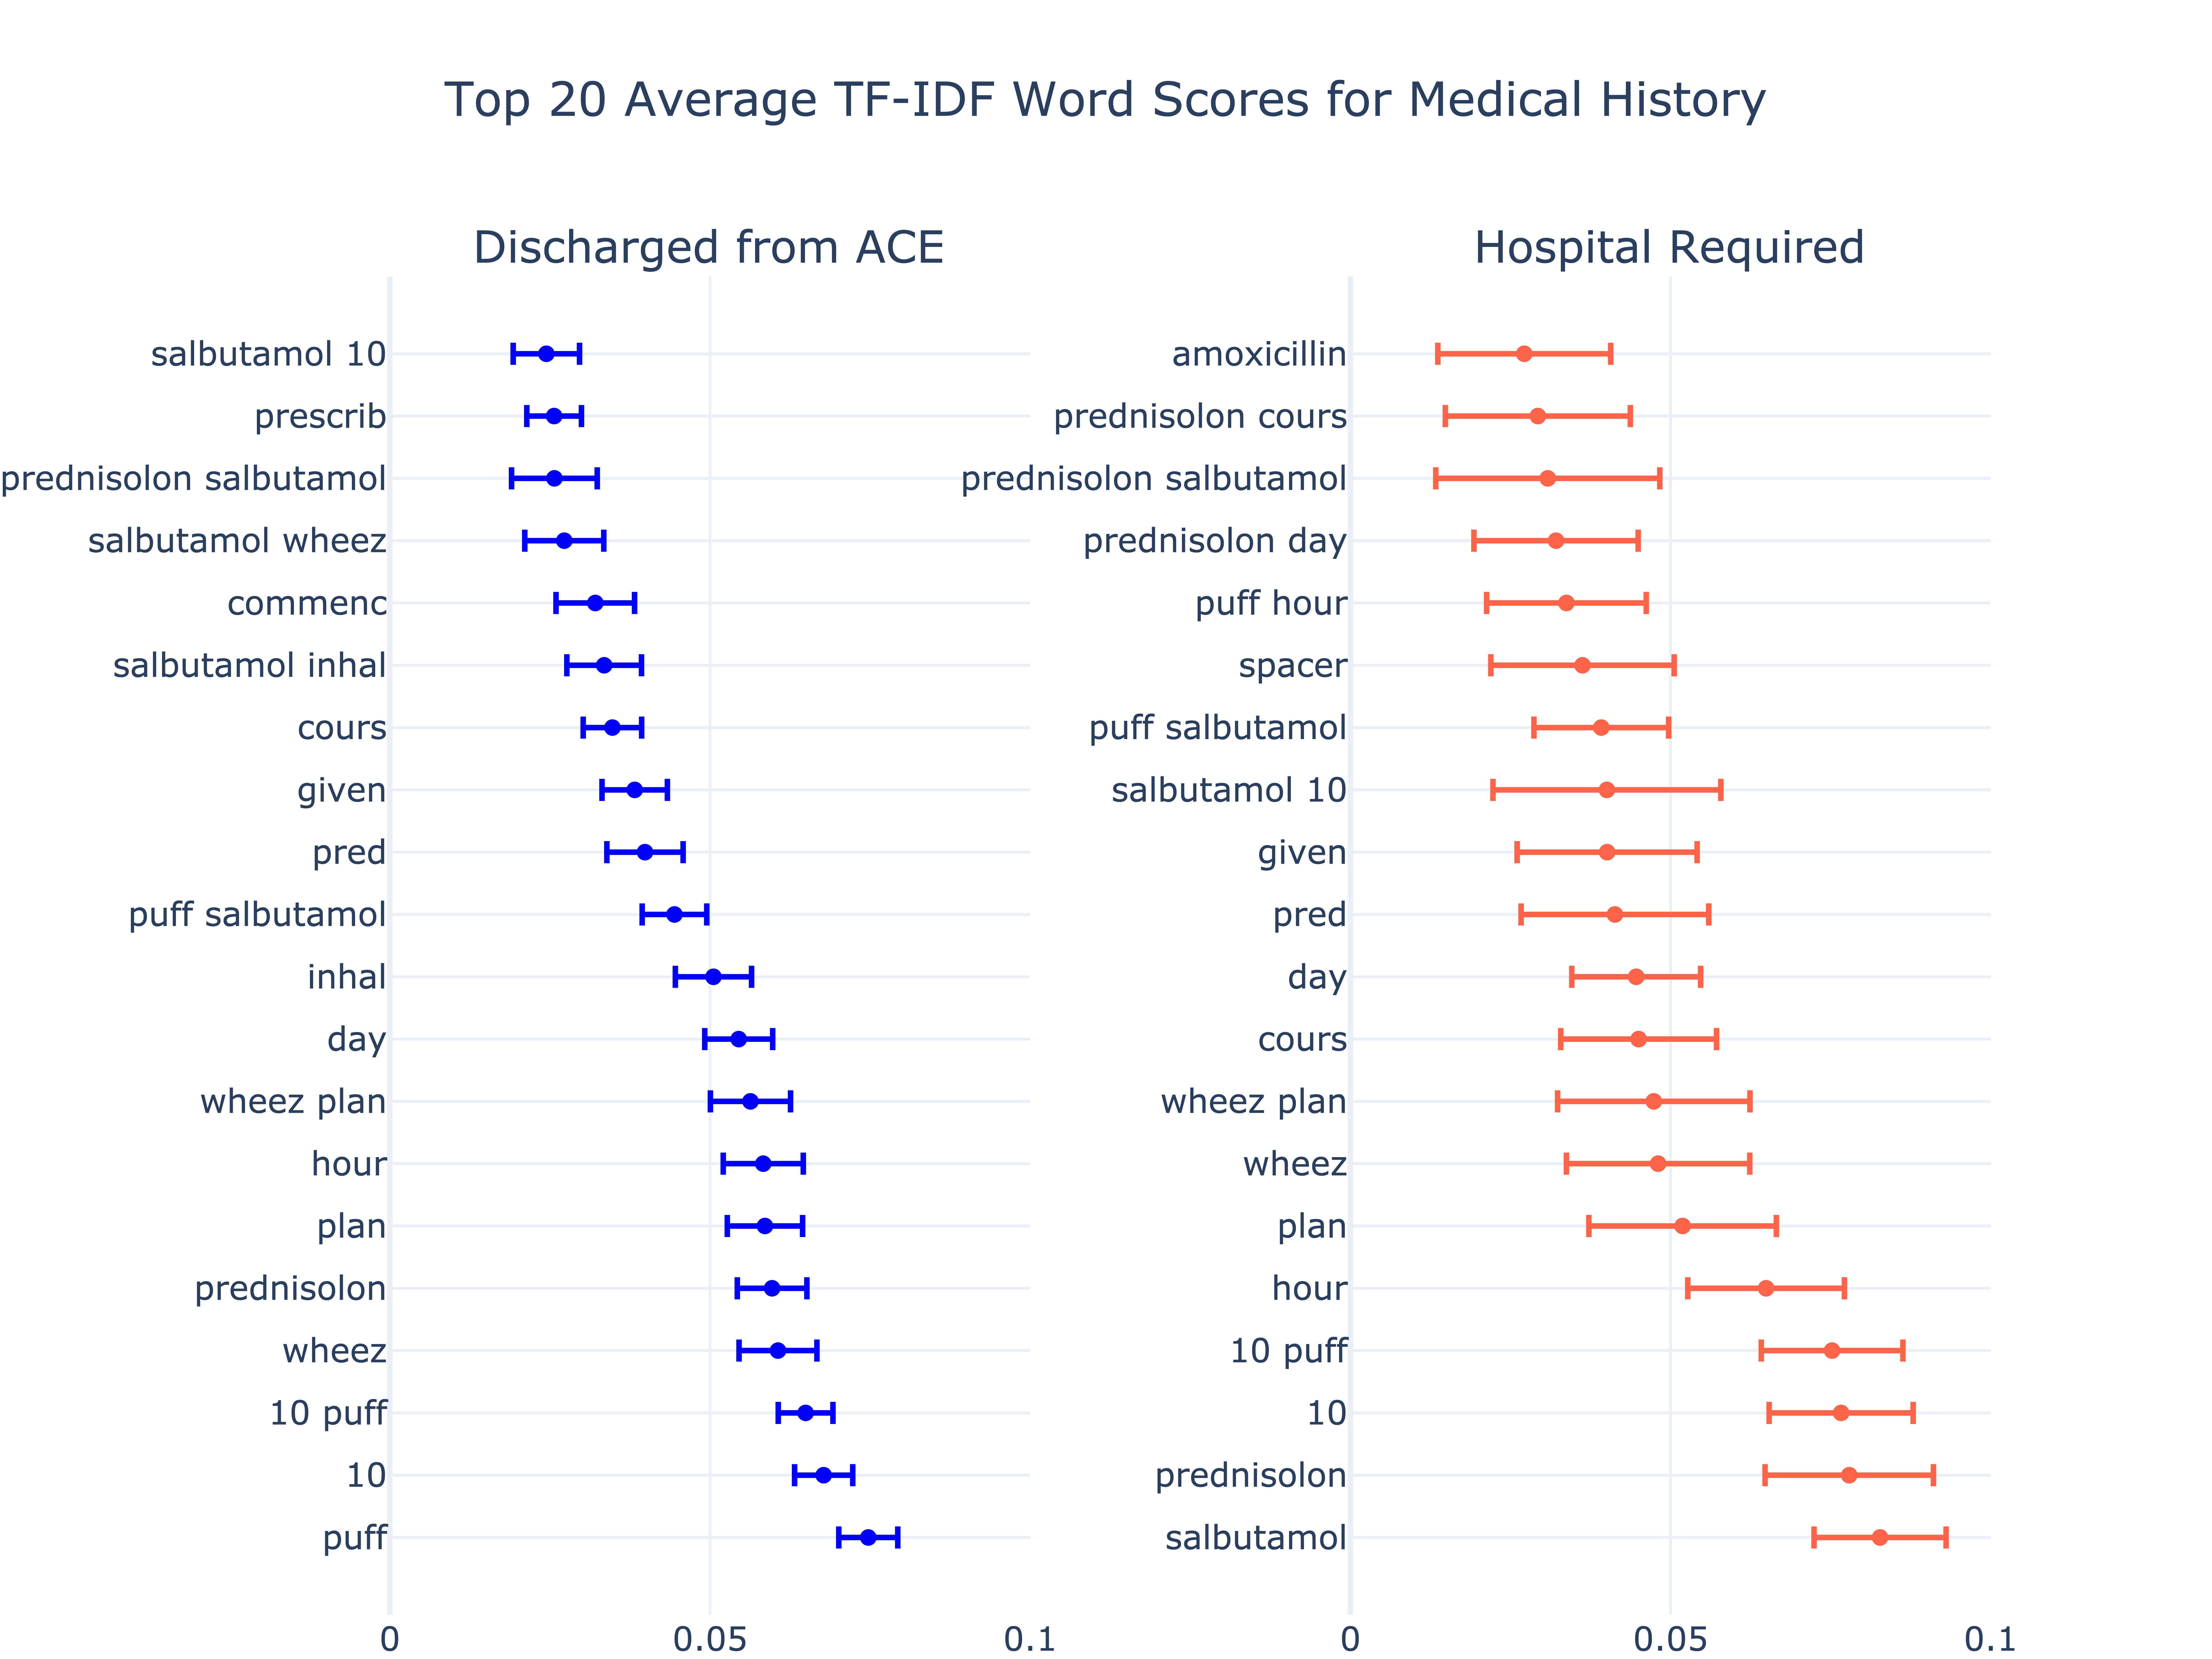
\includegraphics[width=0.9\textwidth]{tf-idf-medical_history}
\end{figure}

\begin{figure}[H]
    \centering
    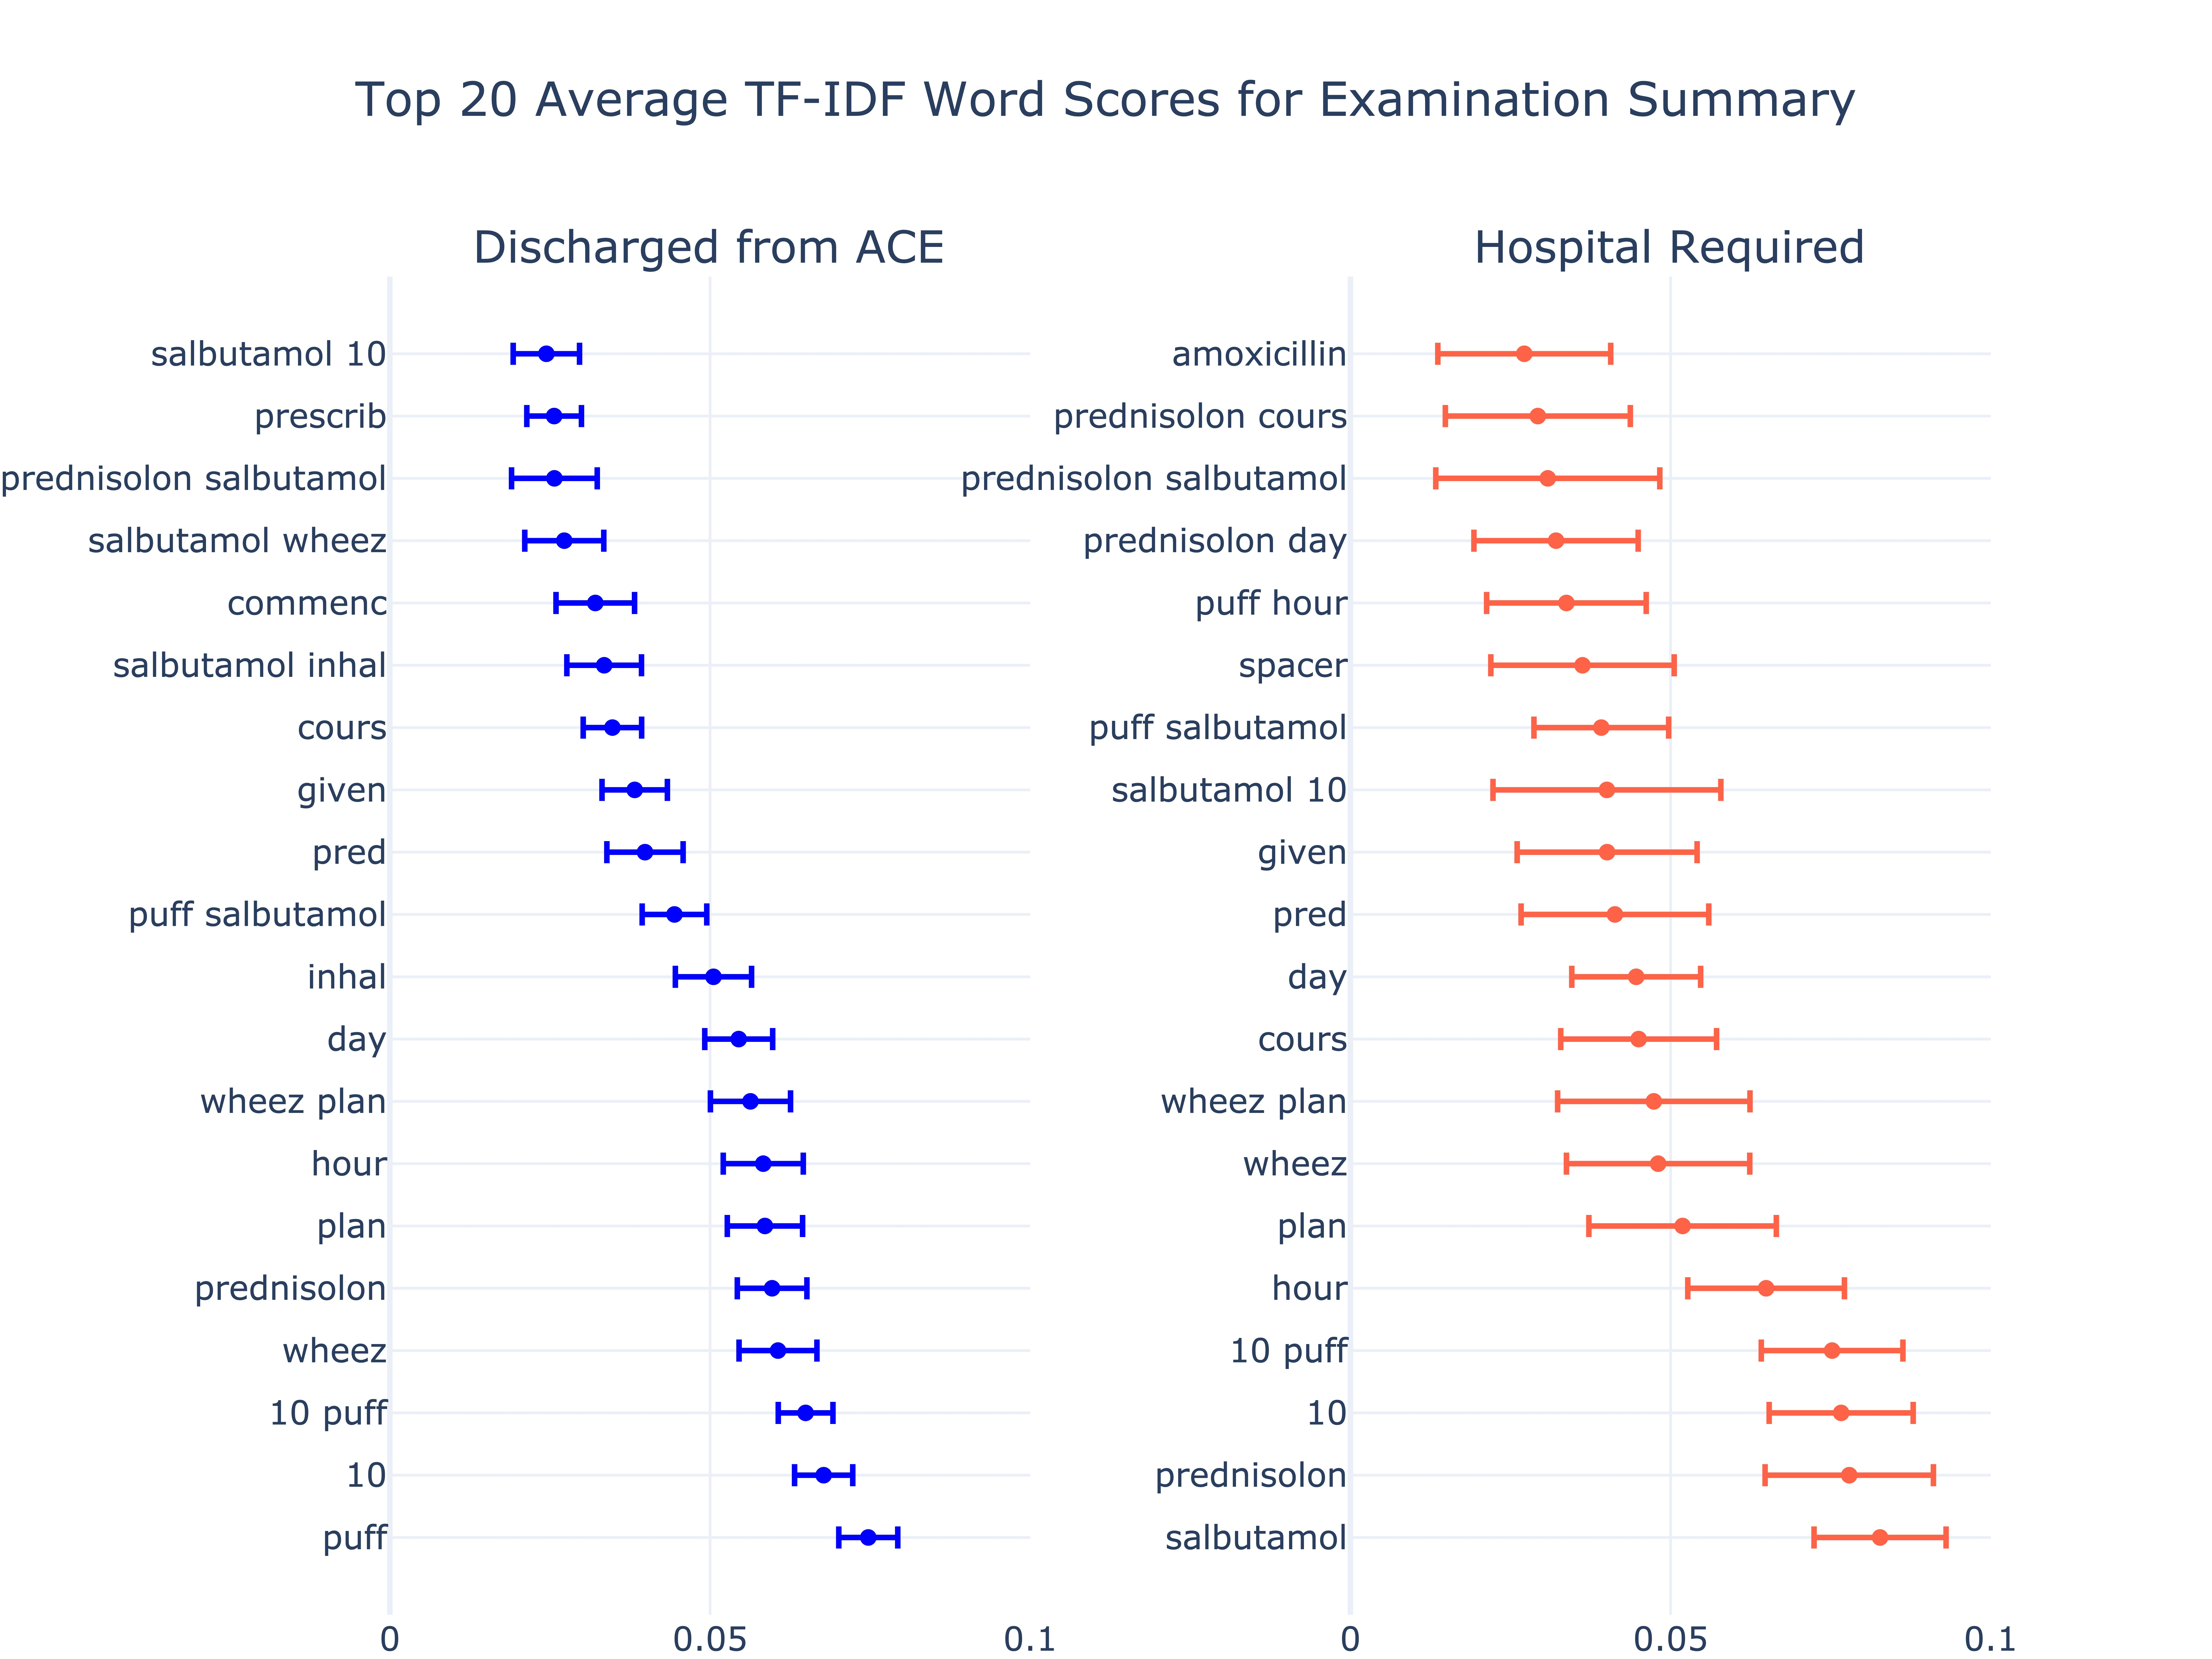
\includegraphics[width=0.9\textwidth]{tf-idf-examination_summary}
\end{figure}

\begin{figure}[H]
    \centering
    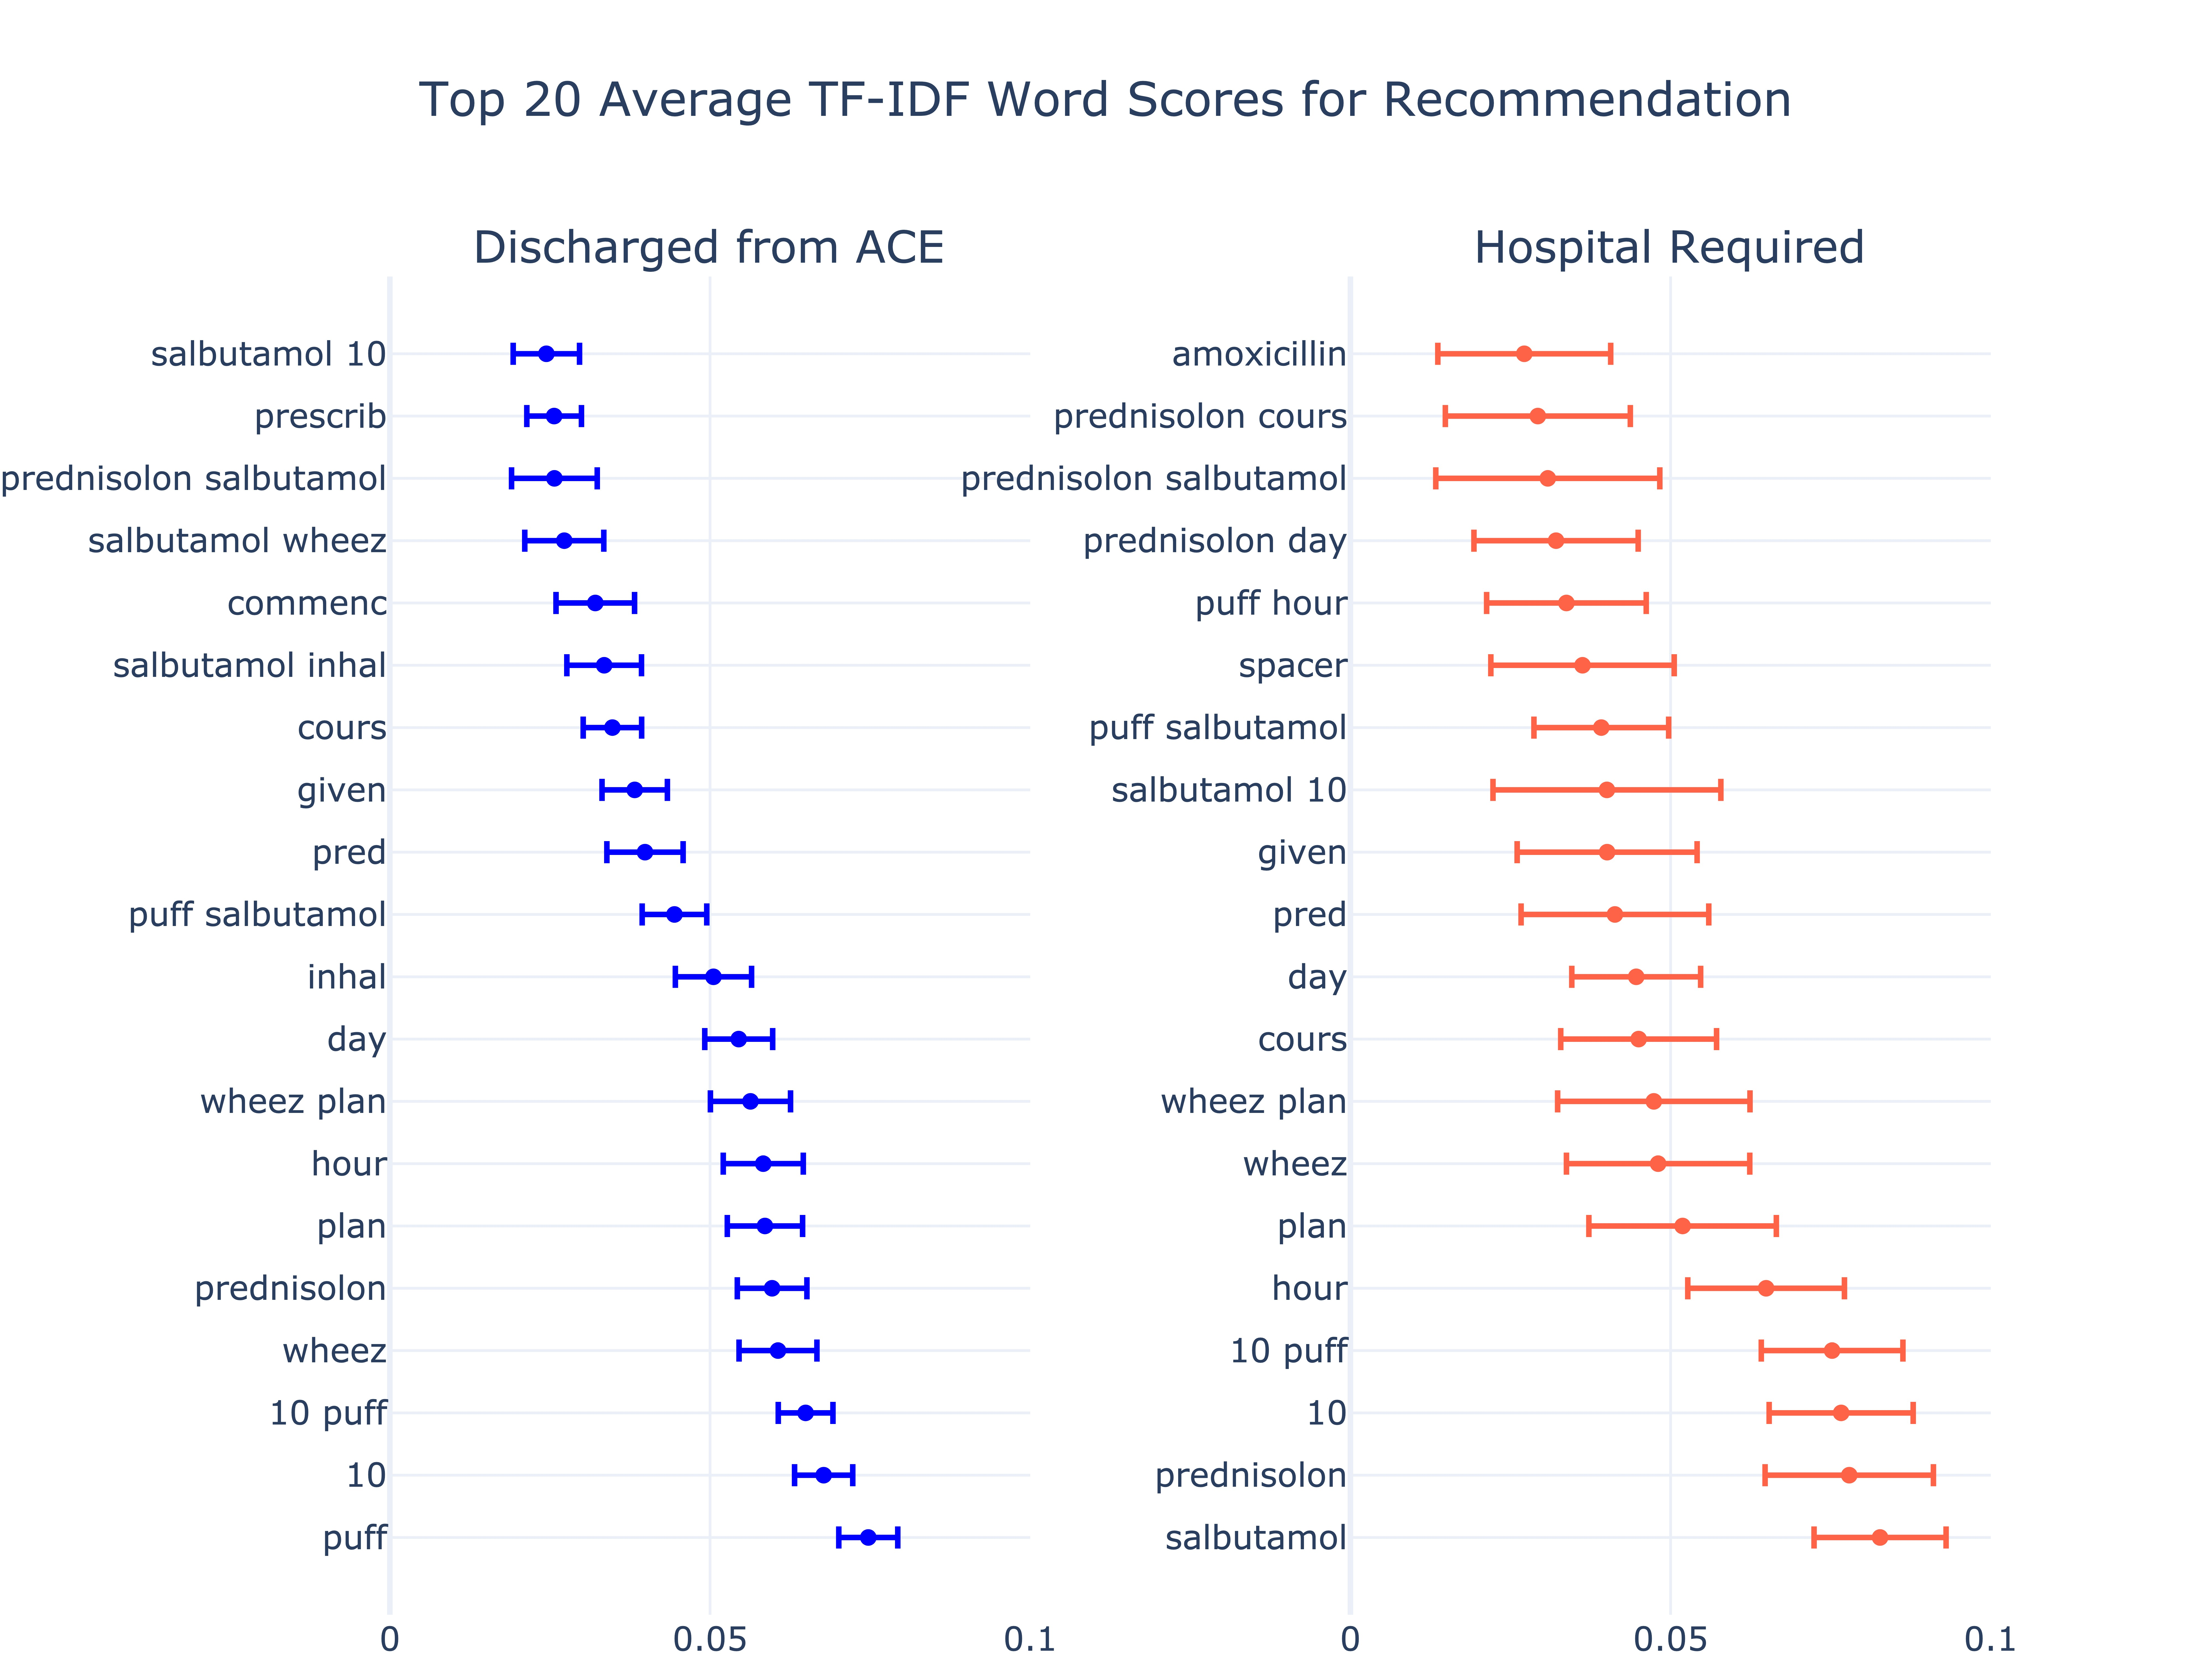
\includegraphics[width=0.9\textwidth]{tf-idf-recommendation}
    \caption[Occurance of TF-IDF scores]{20 highest TF-IDF scores for patients successfully treated by ACE or later referred to hospital. Error bars are the standard errors for each value and hence are much larger for the values taken from patients that required hospital treatment, given that these examples are much fewer in number}
    \label{fig:tf-idf-scores}
\end{figure}

\clearpage
